\chapter{Versuchsdurchführung}

In diesem Kapitel wird der Hardware- und der Softwareafaufbau des Versuches beschrieben.

\section{Versuchsaufbau}

Der Student erhällt folgende Komponenten:
\begin{itemize}
    \item RespberryPi 3
    \item CC2531 Sniffer Stick
    \item cod.m ZigBee CC2652P2 Raspberry Pi Module
    \item 2 x Phillips Hue White E27
    \item 1 x Phillips Hue dimmer switch
    \item HDMI Kabel
    \item Ethernet Kabel
\end{itemize}

Der Student muss KVM Komponenen selbst bereitstellten. Alternativ, wenn der Versuch in der Hochschule durchgeführt werden sollte,
können diese auch durch die Hochschule gestellt werden. Der ZigBee Kordinator ist als \grqq Hat \grqq{} auf dem Raspberry installiert. Der Sniffer ist per USB an der 
Frontseite des Raspberrys angeracht.

\section{Versuchssoftware}

Folgende Software wird eingesetzt:
\begin{itemize}
    \item RaspbianOS
    \item Docker
    \item zigbee2mqtt
    \item mosquitto
\end{itemize}

Auf einem RaspberryPi werden die Anwendungen zigbee2mqtt, Mosquitto sowie HomeAssistant per Docker ausgeführt. Die
Services sind konfiguriert, es sind keine Geräte per Zigbee verbunden. 
Die jeweligen Webinterfaces sind über eine Webadresse im Browser erreichbar. Der ZigBee Kordinator ist als \grqq Hat \grqq{}
auf dem Raspberry installiert. Der Sniffer ist per USB an der Frontseite des Raspberrys angeracht.  

Das Deployment des
Versuchs wird im Kapitel LCM beschrieben.

\section{Aufgabenstellungen}

In diesem Kapitel werden die Aufgabenstellungen aus dem LabGuide genauer beschrieben, sowie eine eine Musterlösung gegeben.


\subsection{Aufgabe 1 - Vertraut machen mit der Umgebung}

\subsubsection{Anmelden am RPI}
Schließen sie an den RaspberryPi einen Monitor, Tastatur, Maus sowie den Sniffer Stick an. Durch anschließen einer
Stromversorgung startet der Raspberry automatisch. Nach einer kurzen Zeit können sie sich mit folgenden Zugangsdaten 
anmelden:

\begin{itemize}
    \item User: Student 
    \item Password: ZigbeeLab
\end{itemize}


Starten sie ein Konsolenfester und überprüfen mit folgendem Befehl, ob die entsprechenden Services laufen:
\begin{lstlisting}
    > docker ps
\end{lstlisting}

Es sollten 3 Container im Status \grqq Running\grqq{} sein. Beschreiben sie in eigenen Worten welche Container sie hier sehen.

\subsubsection{Koordinator Kanal Einstellung}
Starten sie den Webbrowser Firefox und besuchen die Webseite:
\begin{lstlisting}
    https://zigbee2mqtt.local
\end{lstlisting}

Überprüfen, dass keine Geräte mit dem Koordinator verbunden sind. Im Zweifelsfall können sie den Versuch zurücksetzen.
Dies wird in den FAQs beschrieben.

Stellen sie den Kanal, den der Zigbee Koordinator nutzen soll nun auf den durch Ihren Professor vorgegeben Wert.
Dies verhindert, dass sich die Studenten gegenseitig beeinflussen. Zuhause können sie diesen Schritt überspringen.

\begin{figure}[H]
    \centering
    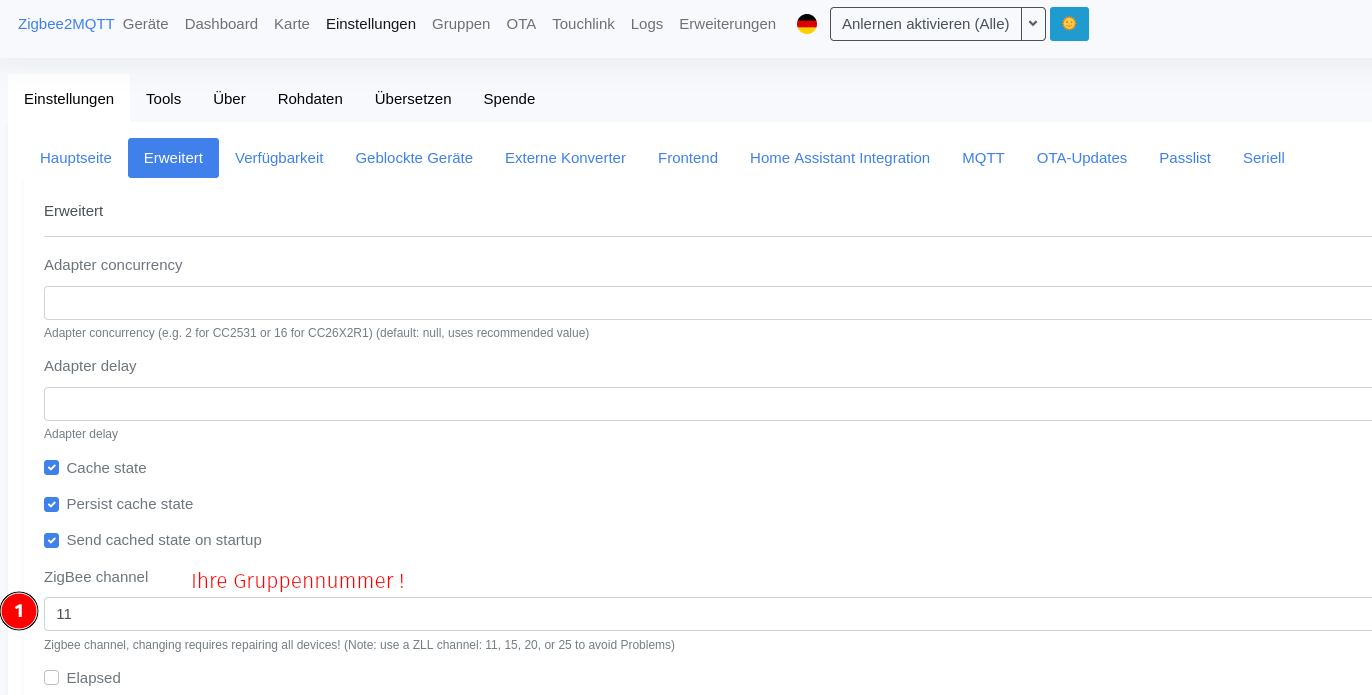
\includegraphics[width=1\textwidth]{media/Z2M-Channel.png}
    \caption{Zigbee Kanal Einstellung}
\end{figure}
Achten sie darauf, im Anschluss die Einstellung am Ende der Seite zu bestätigen. Dafür klicken sie auf den 
\grqq Submit \grqq{} Button am Ende der Seite

\subsubsection{Wireshark Test}
Mit folgendem Befehl können sie ein Wireshak Capture auf entsprechenden Kanal starten:
Starten sie ein Konsolenfester und überprüfen mit folgendem Befehl, ob die entsprechenden Services laufen:
\begin{lstlisting}
    > zbwireshark -c <Kanal>
\end{lstlisting}

Starten sie einen Capture-Vorgang, und beschreiben sie welche Pakete hier sehen.


\subsection{Aufgabe 2 - Joining der Phillips Hue Lampe}

Schalten sie eine der beiden Zigbee Lampen ein. Die Lampe sollte leuchten. Starten sie nun ein Wireshark Capture und
erlauben in zigbee2Mqtt das Anlernen von Geräten. Sobald Zigbee2Mqtt ein erfolgreiches Interview gemeldet hat, beenden sie
den Capture Vorgang. Speichern sie den Wireshark Capture ab.

\begin{figure}[H]
    \centering
    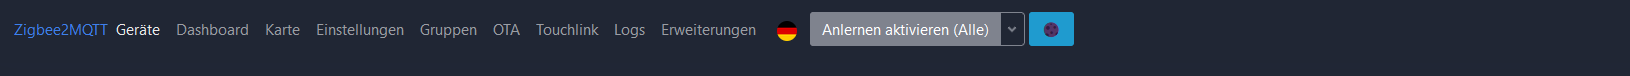
\includegraphics[width=1\textwidth]{media/Z2M-Anlernen.png}
    \caption{Zigbee Kanal Einstellung}
\end{figure}






